\documentclass[tikz]{standalone}

\usetikzlibrary{calc, intersections}

\begin{document}
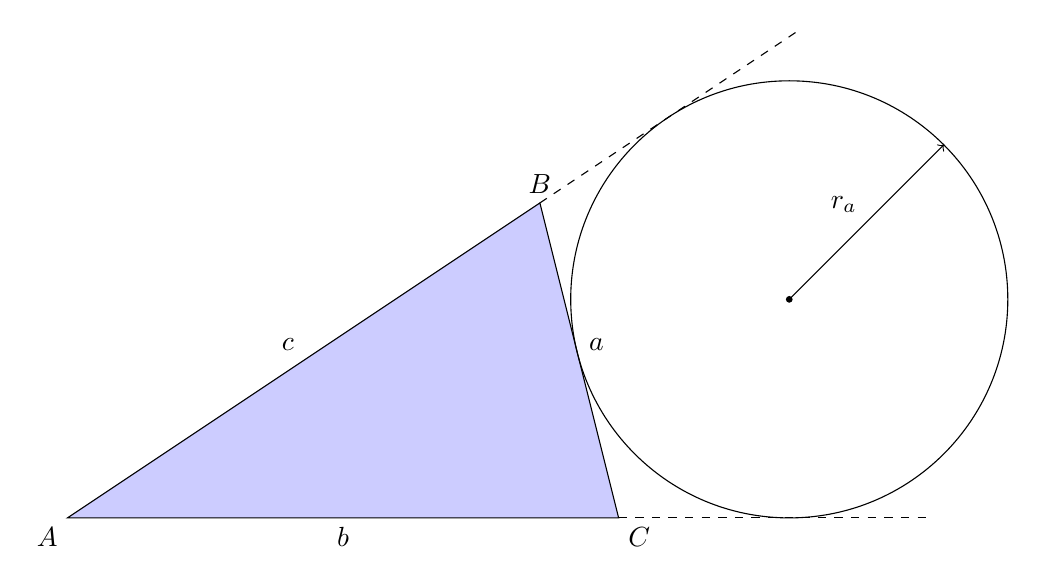
\begin{tikzpicture}

\coordinate (A) at (0,0);
\coordinate (B) at (6,4);
\coordinate (C) at (7,0);

\draw [fill=blue!20] (A) node [below left]{$A$}
      -- node [above left] {$c$} (B) node [above]{$B$}
      -- node [above right] {$a$} (C) node [below right]{$C$}
      -- node [below] {$b$} cycle;

% Define coordinates for excircle opposite vertex A
\coordinate (eA_B_to_C) at ($(B)!1cm!(C)$);
\coordinate (eA_B_to_A_ext) at ($(B)!-1cm!(A)$);
\coordinate (eA_C_to_B) at ($(C)!1cm!(B)$);
\coordinate (eA_C_to_A_ext) at ($(C)!-1cm!(A)$);
\coordinate (eA_B_ext_bis_dir) at ($(eA_B_to_C)!0.5!(eA_B_to_A_ext)$);
\coordinate (eA_C_ext_bis_dir) at ($(eA_C_to_B)!0.5!(eA_C_to_A_ext)$);
\path[name path=eA_B_bisector, overlay] (B) -- ($(B)!30!(eA_B_ext_bis_dir)$);
\path[name path=eA_C_bisector, overlay] (C) -- ($(C)!30!(eA_C_ext_bis_dir)$);

% Find excenter
\draw[name intersections={of=eA_B_bisector and eA_C_bisector, by={excenterA}}];

% Compute exradius
\path let \p1=(A), \p2=(B), \p3=(C) in node[overlay] {
    \def\c{\fpeval{sqrt((\x2-\x1)^2 + (\y2-\y1)^2)}}
    \def\a{\fpeval{sqrt((\x3-\x2)^2 + (\y3-\y2)^2)}}
    \def\b{\fpeval{sqrt((\x3-\x1)^2 + (\y3-\y1)^2)}}
    \def\p{\fpeval{(\c+\a+\b)/2}}
    \def\area{\fpeval{sqrt(\p*(\p-\c)*(\p-\a)*(\p-\b))}}
    \xdef\exradiusA{\fpeval{\area/(\p-\a)}}
};

% Draw circle
\draw (excenterA) circle (\exradiusA pt);

% Show segments
\draw[dashed] (B) -- ($(B)!-4cm!(A)$);
\draw[dashed] (C) -- ($(C)!-4cm!(A)$);

% Show radius of excircle
\def\angle{45}
\draw[fill=black] (excenterA) circle (1pt);
\draw[->] (excenterA) -- node[above left] {$r_a$} ($(excenterA) + (\angle:\exradiusA pt)$);

\end{tikzpicture}
\end{document}
